Practical implementation consists of applying EKF for estimation of 3D position in space, writing a simulation to validate the filter implementation, tuning KF parameters (mainly evaluating covariances) by real-world experiments, testing out whole system and evaluating localization accuracy.

\subsection{Localization}

Describing EKF in detail. Show some code from implementation.

\subsection{Simulation experiments}

\begin{figure}
    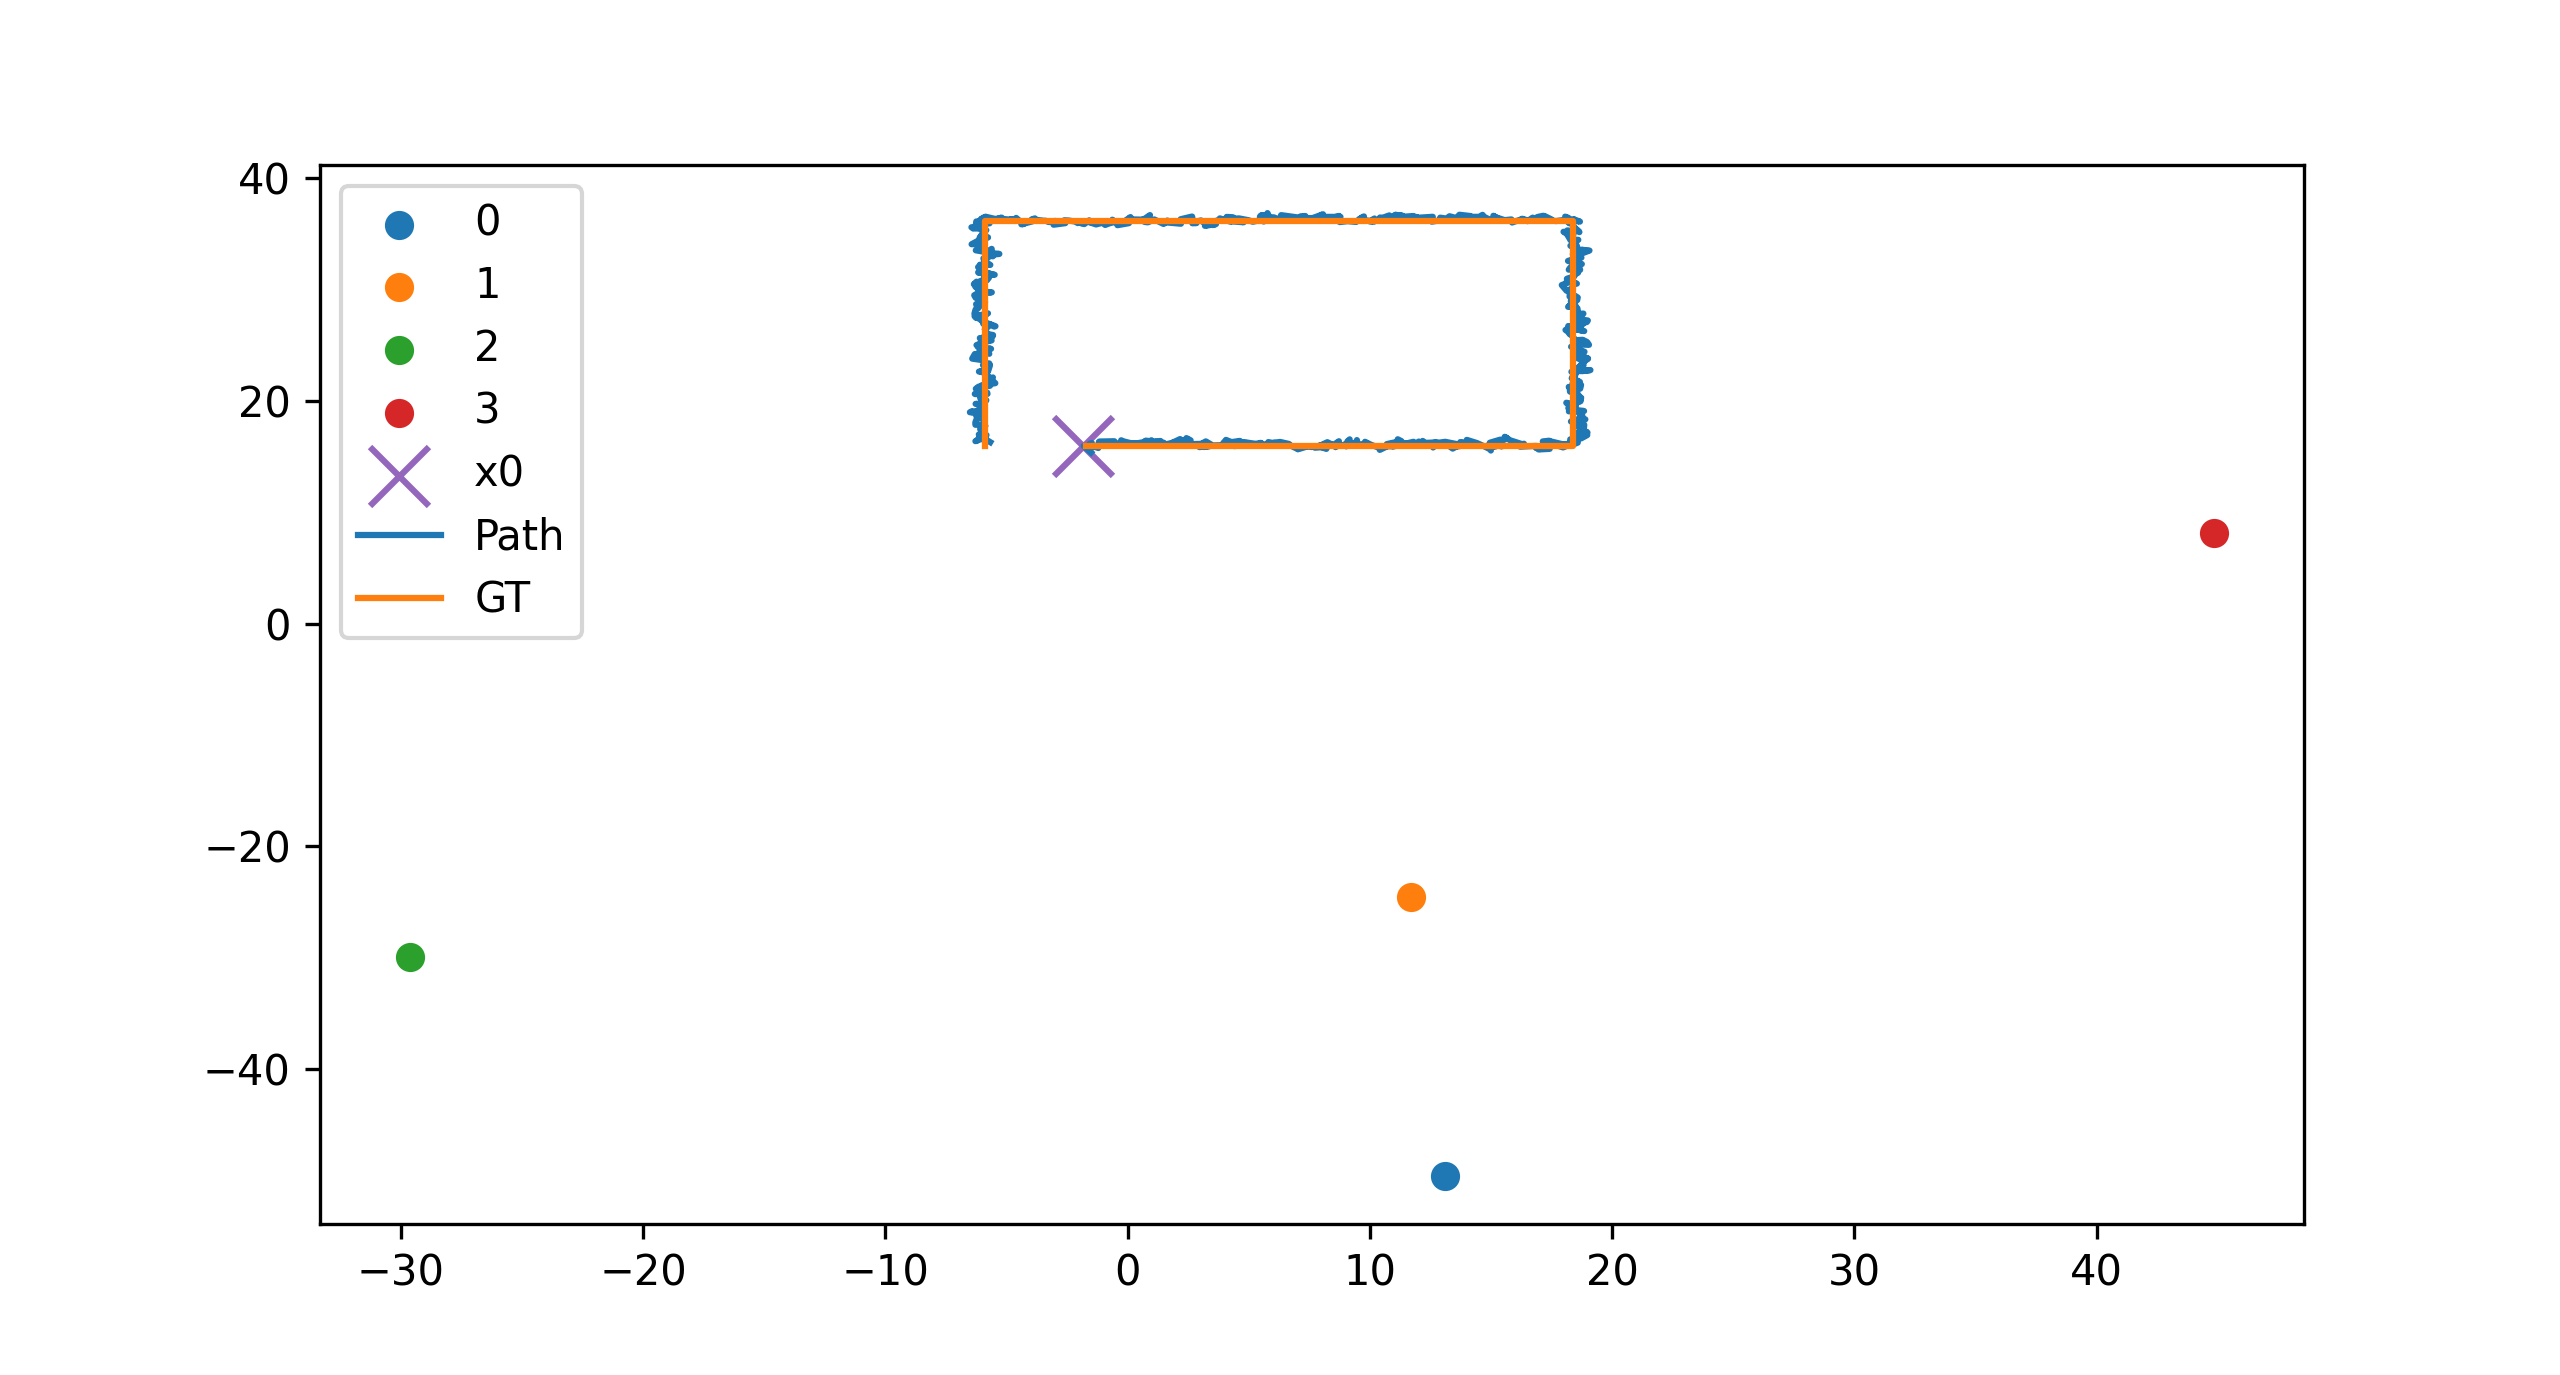
\includegraphics[width=\linewidth]{figures/sim.png}
    \caption{Simulation}
    \label{fig:sim}
\end{figure}

Plots, plots, plots. Noise description?

\subsection{Real-world experiments}

First, it's important to address the assumption made in the simulation environment. It was assumed that sensor measurement variance is known. For filter to have good convergence properties we would like to know it up to a reasonable accuracy level when in operation. Therefore, the first experiment was conducted to measure the precision of UWB range measurements compared to a ground truth. DTU ASTA's Opticon system was used to generate ground truth labels (limited to ~10m range) and two UWB devices, one configured as a tag and another one as an anchor. During the experiment anchor was moved to different position around the track, ground truth distance calculated between devices by taking norm of two position from Opticon and corresponding measurement by the means of UWB antennas was recorded. Figure \ref{fig:distancePDF} shows the probability distributions of measured values by real-world experiments in blue and the ground truth in orange.
\begin{figure}
    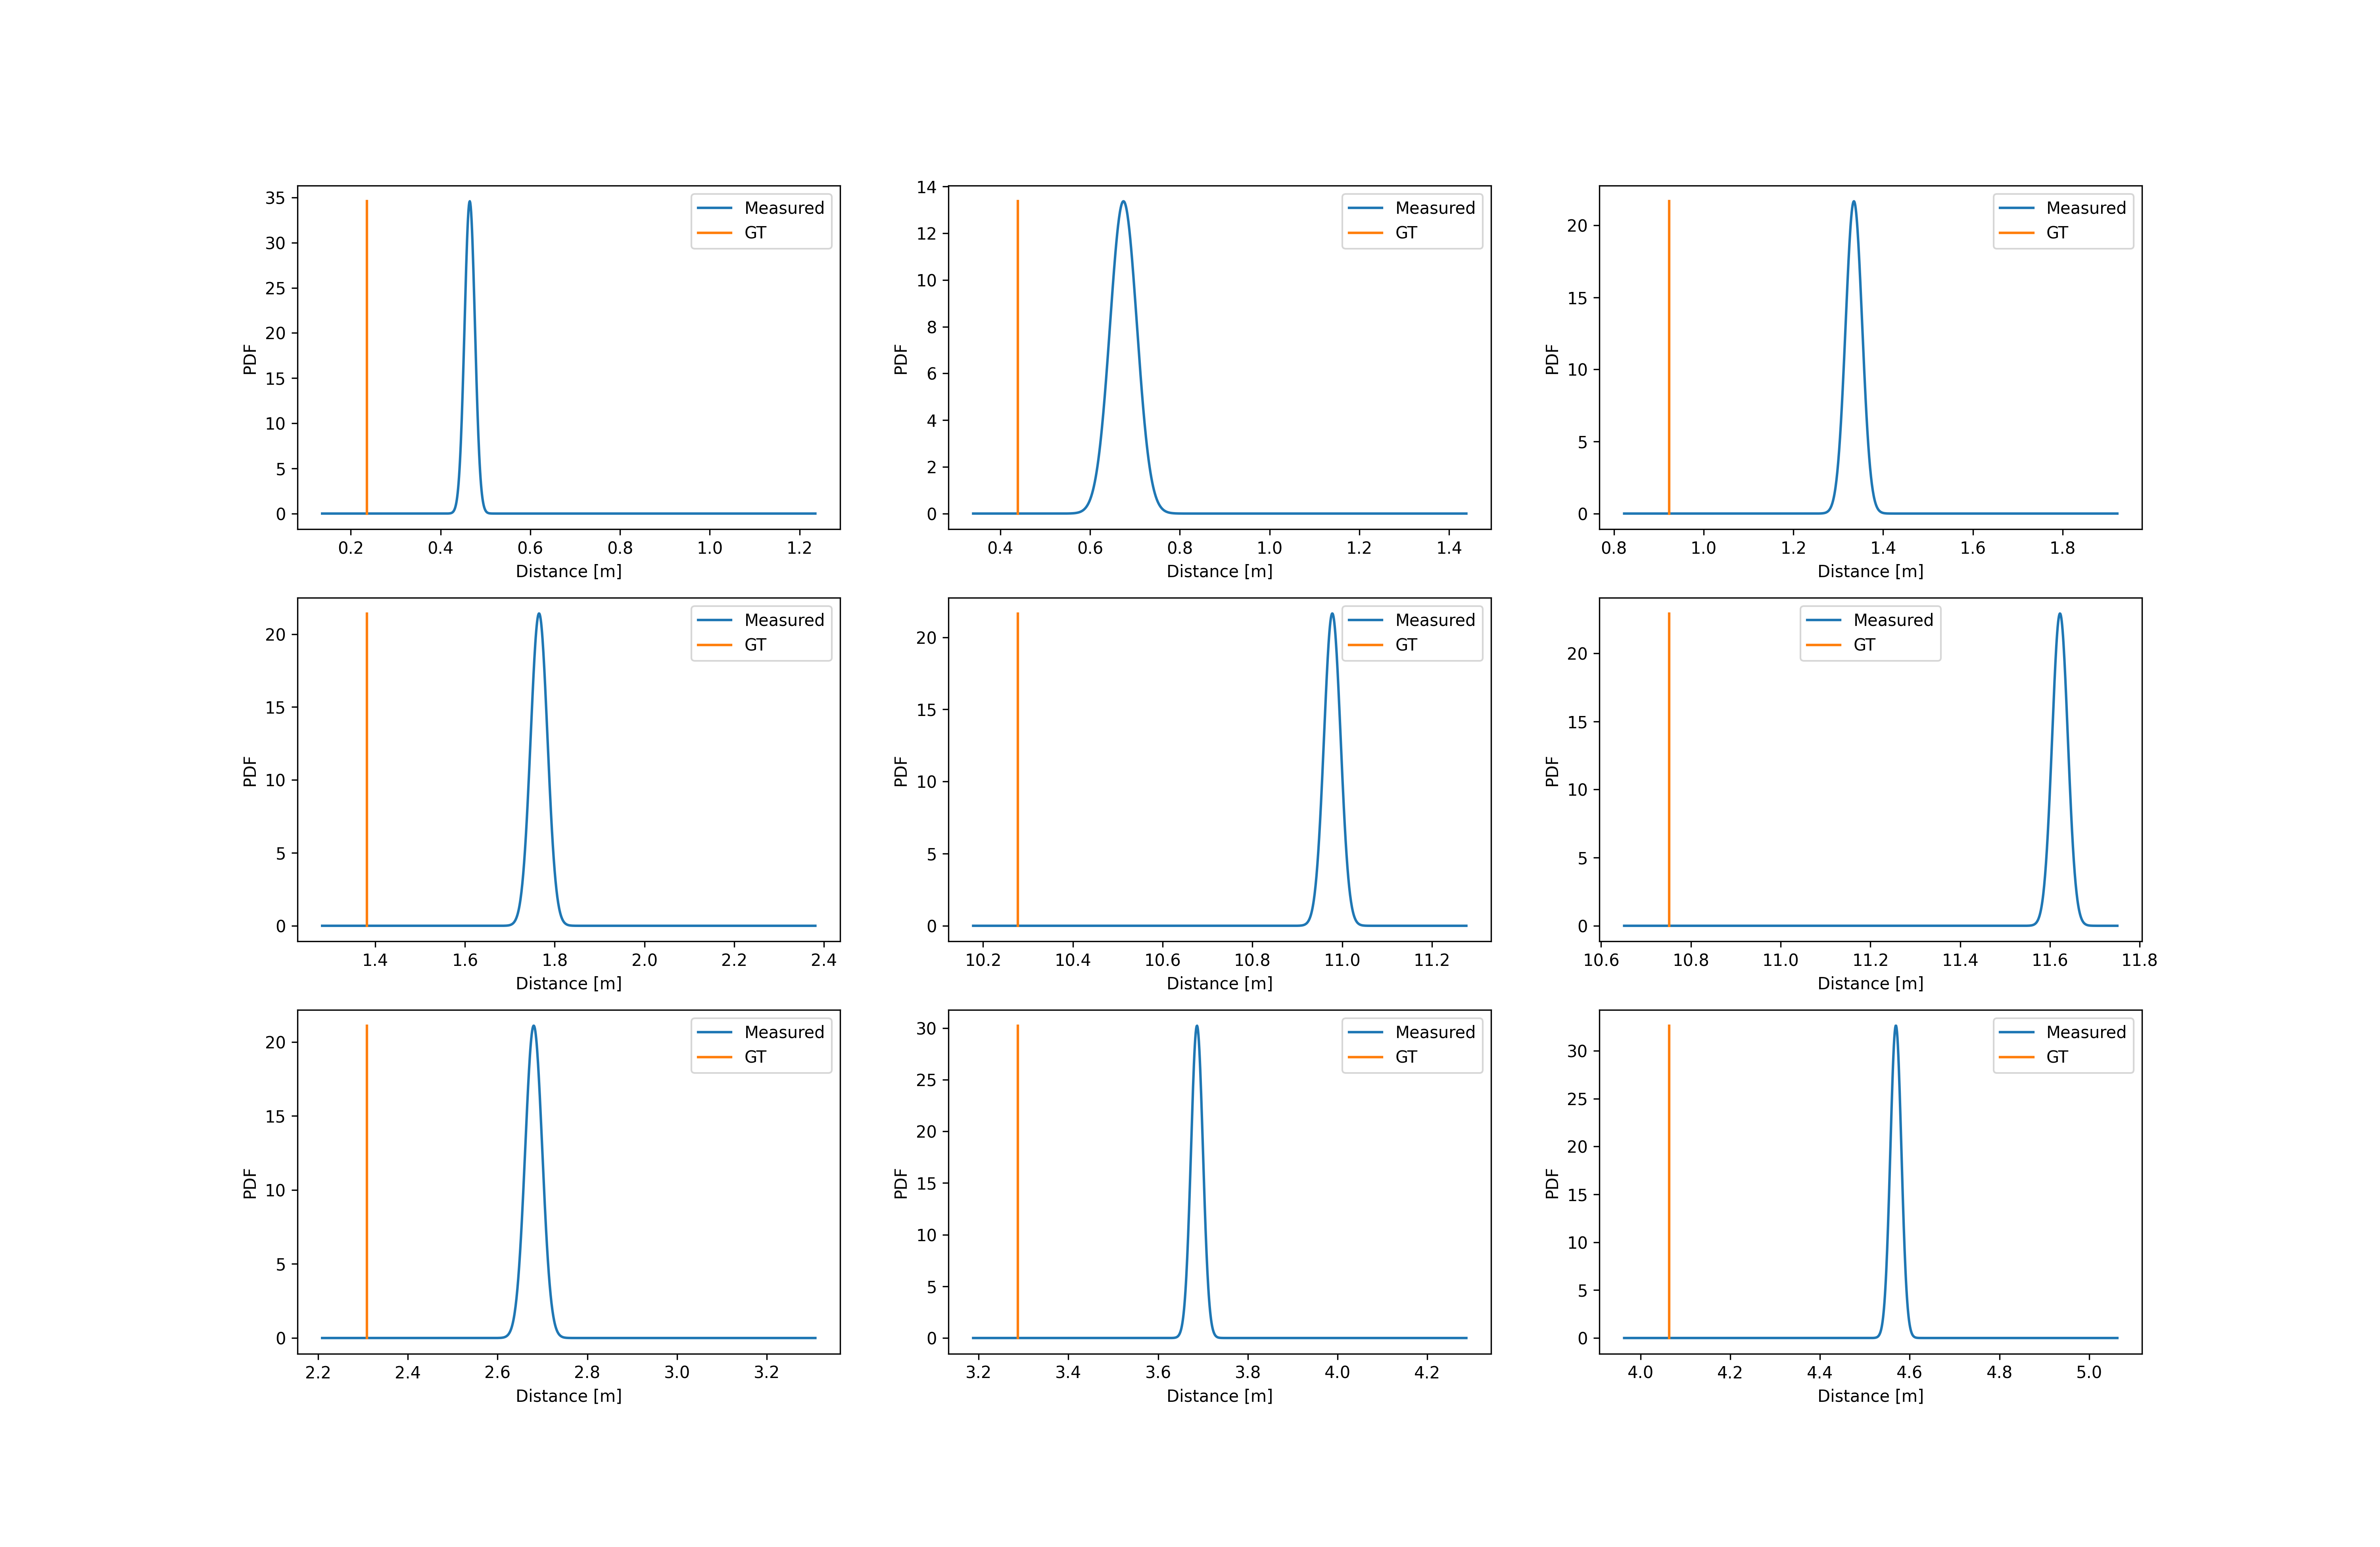
\includegraphics[width=\linewidth]{figures/distancePDF.png}
    \caption{Distance measurements PDFs.}
    \label{fig:distancePDF}
\end{figure}

Looking at the plots one noticeable thing is that mean value of measured values are shifted to the right - meaning sensor gives out bigger distance than it actually is, this could be called bias. The relationship of bias and distance is illustrated in Figure \ref{fig:distance_bias}. Additionally, it can be modeled, at least in this rang,  by a line fit, which is shown in the graph too. It approximates the bias reasonably well and will improve localization accuracy in this distance range. In a way, it's calibrating the sensor so that measurements have the same mean value as ground truths.
\begin{figure}
    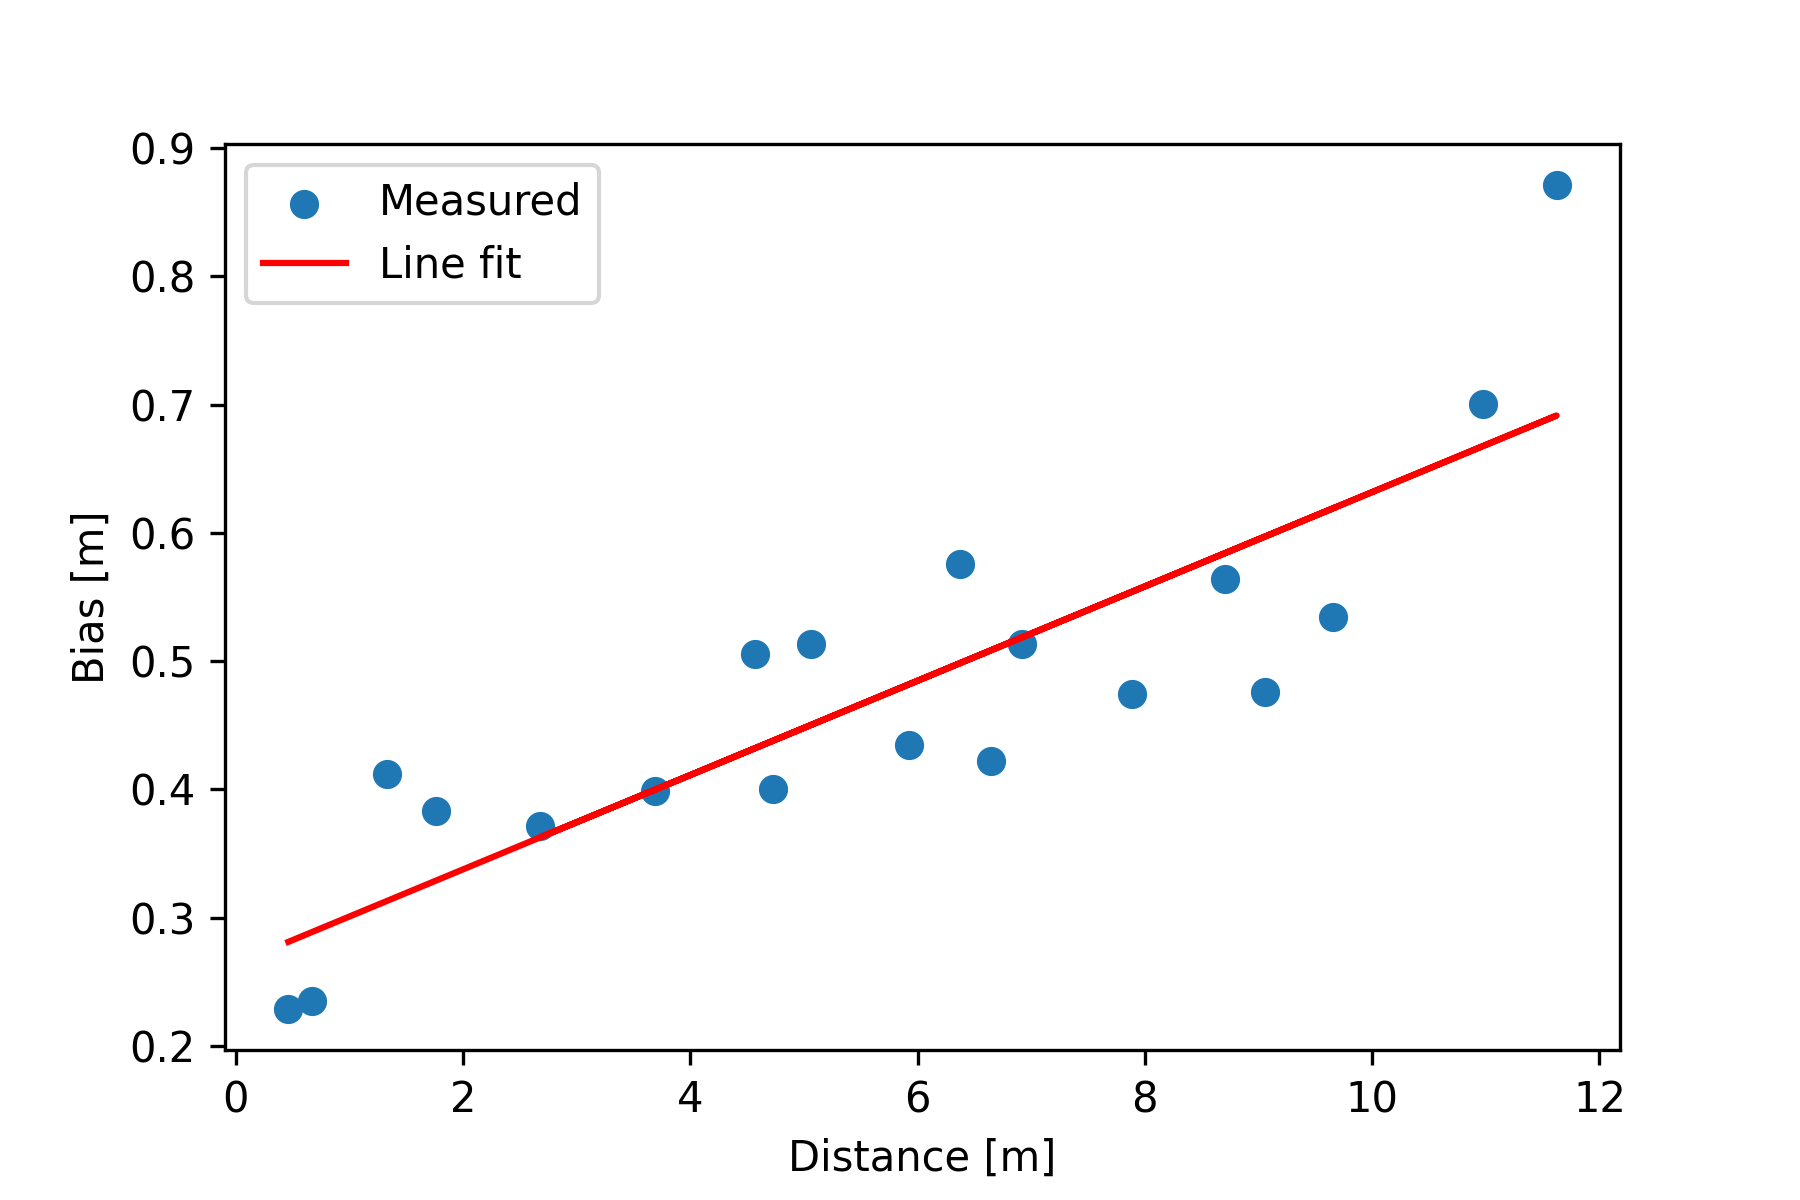
\includegraphics[width=\linewidth]{figures/distance_bias.png}
    \caption{Measurement bias over distance.}
    \label{fig:distance_bias}
\end{figure}

Next, let's look at the variance and distance relation. The question to ask here if they are dependant on each other or we can use single constant values for all range measurements. Figure \ref{fig:distance_var} shows them on single plot, plus a line fir on the data. It's clearly seen that variance is very low and of the same magnitude through out the data points. Thus, we can conclude that under tested conditions constant variance value can be used in EKF. For instance, an average value of all these variance points.
\begin{figure}
    \centering
    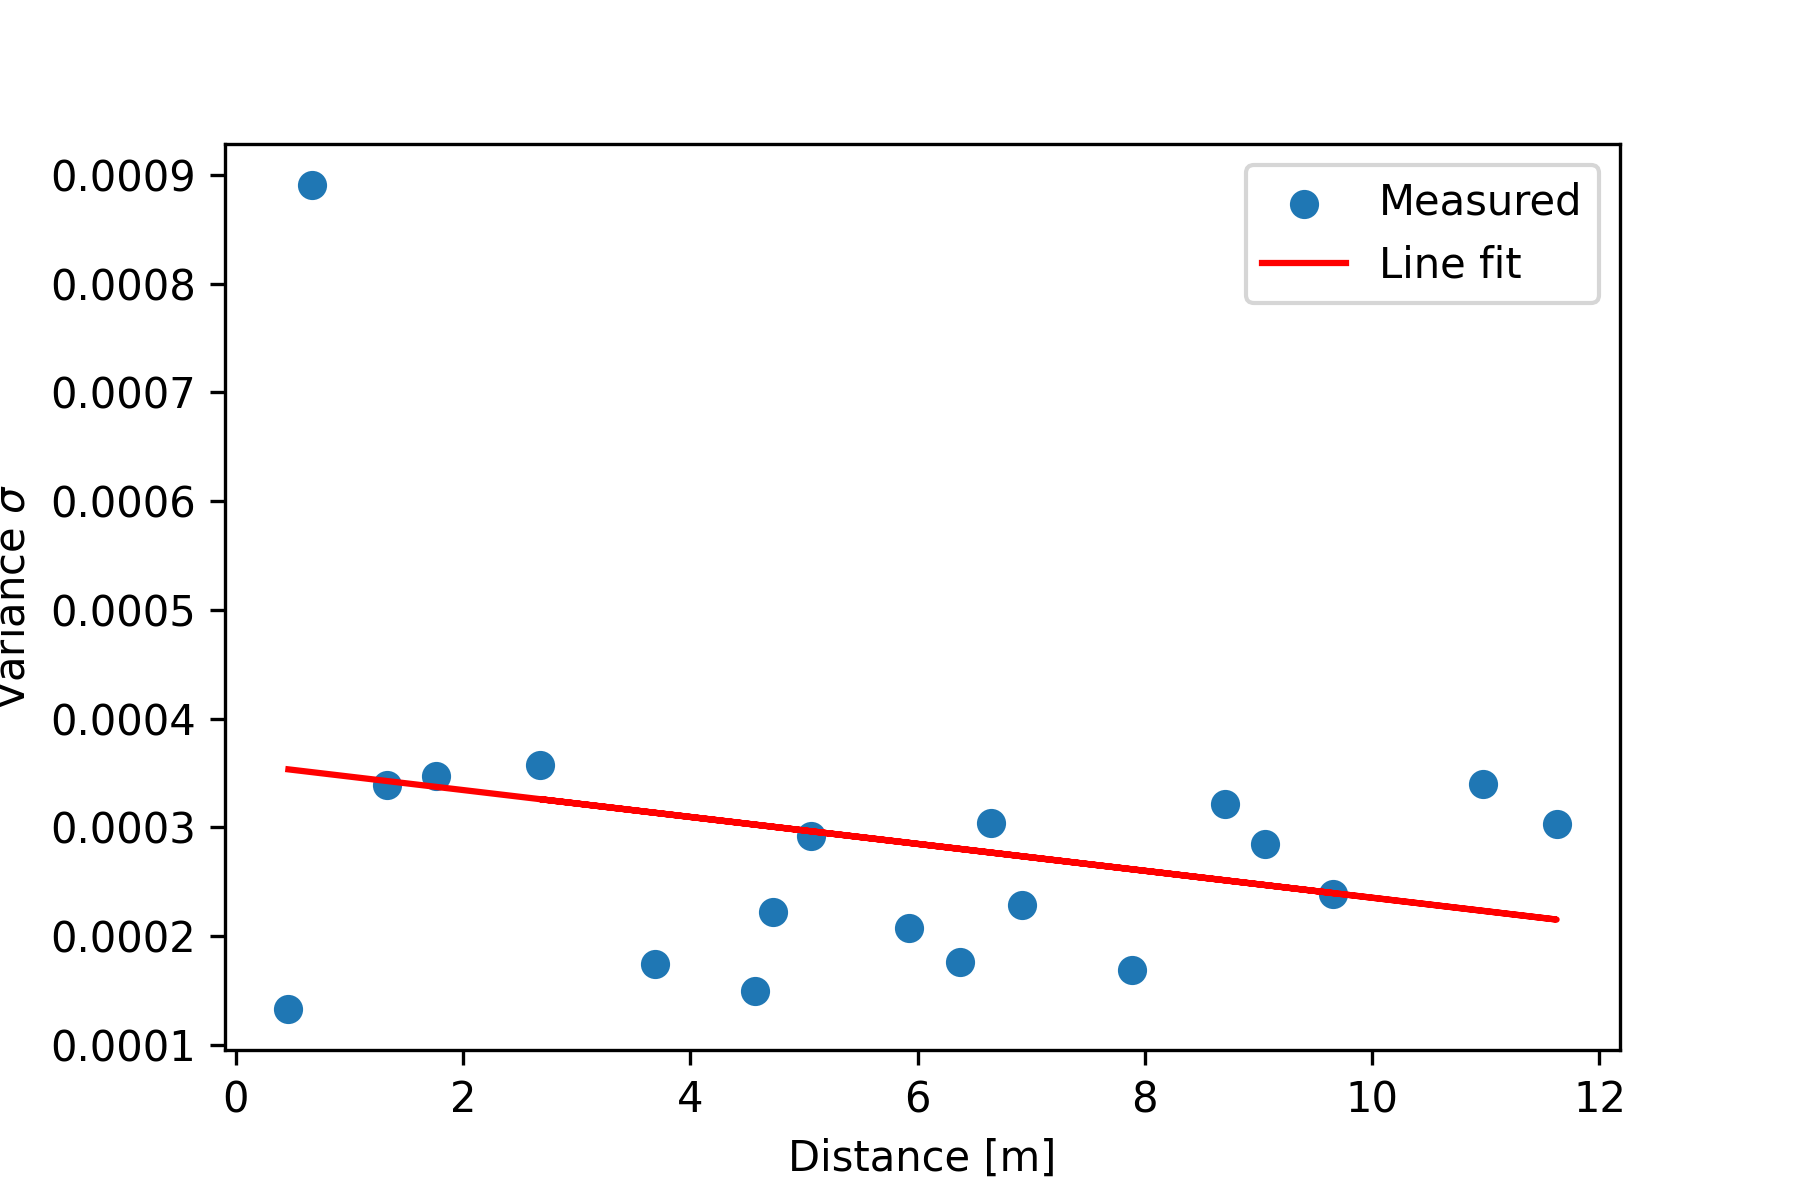
\includegraphics[width=\linewidth]{figures/dist_variance.png}
    \caption{Distance over measurement variance.}
    \label{fig:distance_var}
\end{figure}